\documentclass{tudelft-report}

%% We need to increase the paper size to slightly larger than twice A4 to make
%% room for a front and back cover, including the spine.


\usepackage{fancyhdr}
\usepackage{lipsum}
\usepackage{todonotes}

\usepackage{float}
\usepackage{csquotes}

\usepackage{listings}       % Lstlisting code viewer

\usepackage{longtable}      % Multipage tables

\usepackage{bytefield}

\newcommand{\fakeeighteenbits}[1]{%
    \tiny
    \ifnum#1=1234567890
        #1
    \else
        \ifnum#1<5
            #1%
        \else
            \ifnum#1<13
                $\cdots$%
            \else
                \ifnum#1=13
                    $N-1$
                \else
                    \ifnum#1=14
                        $N$
                    \else
                        \ifnum#1=15
                            $N+1$
                        \else
                            \ifnum#1=16
                                $N+2$
                            \else
                                $N+3$
                            \fi
                        \fi
                    \fi
                \fi
            \fi
        \fi
    \fi
}

\newcommand{\fakeeighteenbitss}[1]{%
    \tiny
    \ifnum#1=1234567890
        #1
    \else
        \ifnum#1<5
            #1%
        \else
            \ifnum#1<13
                $\cdots$%
            \else
                \ifnum#1=13
                    $\cdots$%
                \else
                    \ifnum#1=14
                        $\cdots$%
                    \else
                        \ifnum#1=15
                            $N-2$
                        \else
                            \ifnum#1=16
                                $N-1$
                            \else
                                $N$
                            \fi
                        \fi
                    \fi
                \fi
            \fi
        \fi
    \fi
}

\addtolength{\headheight}{0.9cm} % make more space for the header
\pagestyle{fancyplain} % use fancy for all pages except chapter start
\lfoot{
\includegraphics[height=1.3cm]{figures/colortudelft.png}} % left logo
\rhead{
\includegraphics[height=1.3cm]{figures/projectluna.png}} % right logo
\renewcommand{\headrulewidth}{0pt} % remove rule below header

\setlength\parindent{0pt}       % Do not indent a new paragraph

\def\iic{\texorpdfstring{I$^2$C}{I2C}}  % I2C text format


\definecolor{darkpink}{rgb}{1.0, 0.13, 0.32}


\lstdefinestyle{DOS}
{
    backgroundcolor=\color{black},
    basicstyle=\scriptsize\color{white}\ttfamily
}


\begin{document}
%% Use Roman numerals for the page numbers of the title pages and table of
%% contents.
% \frontmatter

%% Uncomment following 19 lines for a cover with a picture on the lower half only
\title[tudelft-white]{Bus Manager}
\subtitle[tudelft-cyan]{Lunar Zebro}
\author[tudelft-white]{Software Department}
\affiliation{-}
\coverimage{figures/page1background.png}
\titleoffsetx{2cm}
\titleoffsety{8cm}
\afiloffsetx{1cm}
\afiloffsety{18cm}
\covertext[tudelft-white]{
    \textbf{Cover Text} \\
    possibly \\
    spanning
    multiple
    lines
    \vfill
    ISBN 000-00-0000-000-0
}
\setpagecolor{black}
\makecover



%
%% Include an optional title page.
\begin{titlepage}


\begin{center}

%% Insert the TU Delft logo at the bottom of the page.

%% Print the title in cyan.
{\makeatletter
\largetitlestyle\fontsize{64}{94}\selectfont\@title
%\largetitlestyle\color{tudelft-cyan}\Huge\@title
\makeatother}

%% Print the optional subtitle in black.
{\makeatletter
\ifx\@subtitle\undefined\else
    \bigskip
   {\tudsffamily\fontsize{22}{32}\selectfont\@subtitle}
    %\titlefont\titleshape\LARGE\@subtitle
\fi
\makeatother}

\bigskip
\bigskip

by
%door

\bigskip
\bigskip

%% Print the name of the author.
{\makeatletter
%\largetitlefont\Large\bfseries\@author
\largetitlestyle\fontsize{26}{26}\selectfont\@author
\makeatother}

\bigskip
\bigskip

in partial fulfilment of the requirements for documentation for:
%ter verkrijging van de graad van Master of Science

TU Delft, The Netherlands
%aan de Technische Universiteit Delft,

%to be defended publicly on Tuesday January 1, 2013 at 10:00 AM.
%in het openbaar de verdedigen op dinsdag 1 januari om 10:00 uur.

\vfill

\begin{tabular}{lll}
    Project Director: & prof. dr. ir. C. J. M. Verhoeven, & TU Delft \\
    System Engineer: & Pranav Gurumallappa, & TU Delft \\
    Operations Manager: & Maneesh Verma, & TU Delft \\
%    Project duration: & \multicolumn{2}{l}{March 1, 2012 -- January 1, 2013} \\
    Head of Software: & dr. A. Noroozi, & TU Delft \\
    Vice Head of Software: & Y. Klaassens, & TU Delft \\
\end{tabular}
%% Only include the following lines if confidentiality is applicable.

\bigskip
\bigskip
\emph{This document is confidential and cannot be made public unless a written permission has been obtained from project director.
}
%\emph{Op dit verslag is geheimhouding van toepassing tot en met 31 december 2013.}

\bigskip
\bigskip
%An electronic version of this thesis is available at %\url{http://repository.tudelft.nl/}.
%\\[1cm]

%\centering{
\includegraphics{cover/logo_black}}


\end{center}

\begin{tikzpicture}[remember picture, overlay]
    \node at (current page.south)[anchor=south,inner sep=0pt]{
        
\includegraphics{cover/logo_black}
    };
\end{tikzpicture}

\end{titlepage}


\tableofcontents

%% Use Arabic numerals for the page numbers of the chapters.
% \mainmatter

\chapter{Introduction}
Because RS485 is a half-duplex protocol, software on both ends of the physical data line should follow the same set of rules defined in the protocol and Message Format (see Chapter \ref{ch:message_format}). The Bus Manager is responsible for transferring commands and data between subsystems while adhering to this format.
This implies checking for CRC errors and sending a retransmission request or NACK when it needs to do so.
The Bus Manager acts between the Application Layer and the Physical Layer of the OSI model.

Figure \ref{fig:rs485_diagram} shows that there are 5 different RS485 buses inside the rover.
The Bus Manager also prevents any race condition on its assigned bus and makes sure that multiple apps cannot communicate with their subsystem at the same time.
\todo[inline]{Not sure about this yet}

\begin{figure}[H]
    \centering
    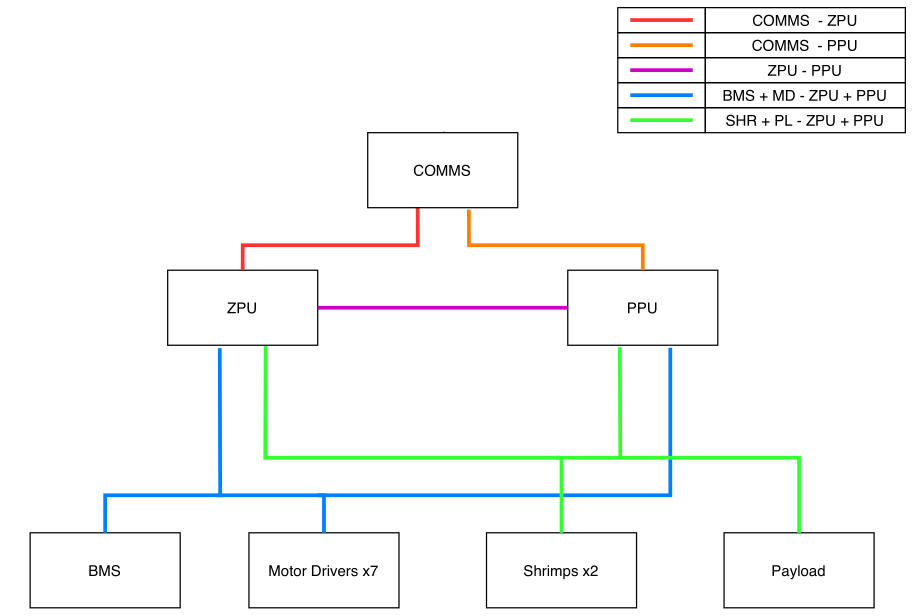
\includegraphics[scale=0.4]{figures/RS485_connections.png}
    \caption{Schematic view of the physical RS485 busses layout}
    \label{fig:rs485_diagram}
\end{figure}


\newpage


It is a bit awkward and impractical to uniquely identify RS485 buses based on the colours used in Figure \ref{fig:rs485_diagram}.
This is why we map the colours of Figure \ref{fig:rs485_diagram} to a unique bus name and number.
Table \ref{tab:buslegend} shows this mapping.
From now on in this document as well as in code, we will refer to bus names rather than bus colours.

\definecolor{amethyst}{rgb}{0.6, 0.4, 0.8}
\definecolor{bleudefrance}{rgb}{0.19, 0.55, 0.91}

\begin{longtable}{| p{0.1\textwidth} | p{0.15\textwidth} | }
    \hline
    \textcolor{red}{Bus name} & \textcolor{red}{Bus colour} \\
    \hline
    Bus0 & 
\begin{tikzpicture} \draw[line width=1mm, color=red] (0,0) -- (2,0); \end{tikzpicture} \\
    \hline
    Bus1 & 
\begin{tikzpicture} \draw[line width=1mm, color=orange] (0,0) -- (2,0); \end{tikzpicture} \\
    \hline
    Bus2 & \begin{tikzpicture} \draw[line width=1mm, color=amethyst] (0,0) -- (2,0); \end{tikzpicture} \\
    \hline
    Bus3 & \begin{tikzpicture} \draw[line width=1mm, color=bleudefrance] (0,0) -- (2,0); \end{tikzpicture} \\
    \hline
    Bus4 & 
\begin{tikzpicture} \draw[line width=1mm, color=green] (0,0) -- (2,0); \end{tikzpicture} \\
    \hline

    \caption{Bus legend mapping bus names to colours}
    \label{tab:buslegend}
\end{longtable}


\section{Background information and History}

\subsection{First version (1.0)}
Bus Manager is a concept that was first introduced in February 2021 as part of Max' thesis \cite{comms_thesis}.
Between February 2021 and August of 2021, the foundational layer of Bus Manager was laid which includes, but is not limited to, the Message Format.
Unit tests have shown that this first revision of Bus Manager used to work.

\subsection{Second version (2.0)}
In the second revision of Bus Manager, a few modifications have been made.
One of these changes is, for instance, that the Bus Manager won't send an initial message to request if an $x$ amount of bytes are available for the receiver to receive. Instead, it will just send the command which includes the length as part of the Message Format.
\todo[inline]{Clear up this sentence}
\par The second revision also uses a semaphore to synchronise bus access between bus managers, because the idea was for each subsystem app to have its own bus manager.

\subsection{Third version (2.1)}
The third version of the Bus Manager uses a more centralised approach. The Bus Managers live on the OBC in their own app, which coordinates bus access for all buses. Apps need to communicate with the Bus Managers via inter-thread communication. This avoids the need for using shared semaphores and decreases the dependencies between the subsystem apps. For further information about the design, see Chapter \ref{ch:design}.


\section{List of features of Bus Manager 2.1}

Now that the reader is aware of the overall functionality of the Bus Manager, we can list a set of features that characterises Bus Manager 2.1 (subject to change).

\begin{itemize}

    \item{\textbf{Instances}. Each bus has a separate instance of the Bus Manager that manages the access to that bus. Avoids the need for a more complex solution for all buses.}

    \item{\textbf{Timeout}. When a Bus Manager sends any type of message it waits for a response. A configurable timeout limit can be set to signal an error if the response is not received within that limit. }

    \item{\textbf{Retries}. When too many timeouts have happened and \textbf{<tbd>} retries are exceeded, then the application layer of this particular Bus Manager is informed about the failure.}

    \item{\textbf{Portability}. Because of the extensive use of Bus Manager both on the masters (OBC, PPU) and slaves (subsystems), it is of extra interest to design and implement Bus Mananger in such a way that it is easy to port over to subsystems which run different hardware architectures. Reimplementing it means that subsystem designers need to be fully aware of the protocol- and Message Format and this is a source of error and requires extra testing and validating. Bus Manager should be easily portable and be abstract in nature.}

    \item{\textbf{Sustainability}. Bus Manager shall comply to the Lunar Zebro Software guidelines. These include, but are not limited to: the code style guide and GoogleTest Unit Tests. The Git repository follows the same skeleton as all the other software modules.}

\end{itemize}


\chapter{Appendix}

\section{Known bugs and issues}

This section will list all known bugs and issues encountered during the development of the firmware.


%% Use letters for the chapter numbers of the appendices.
\appendix

%\input{appendix-a}

\bibliography{report}




\end{document}
